\subsection{R Syntax}
\makesubcontentsslidessec


\begin{frame}
  \begin{block}{Data Types}\pause
  \begin{itemize}[<+-|alert@+>]
    \item Storage:  logical, int, double, double complex, character
    \item Structures:  vector, matrix, array, list, dataframe
    \item Caveats:  (Logical) \code{TRUE}, \code{FALSE}, \code{NA}
  \end{itemize}
  For the remainder of the tutorial, we will restrict ourselves to real number 
matrix computations.
\end{block}
\end{frame}

% \begin{frame}
%   \begin{block}{Other notable }\pause
%   \begin{itemize}[<+-|alert@+>]
%     copy on write, lexical scoping, column major
%   \end{itemize}
% \end{block}
% \end{frame}



\begin{frame}[fragile]
  \begin{block}{Basics (1 of 2)}\pause
  \begin{itemize}[<+-|alert@+>]
    \item The default method is to print:
    \vspace{-.4cm}
    
\begin{lstlisting}[backgroundcolor=\color{white},basicstyle=\ttfamily\color{
dkgray}\scriptsize,keywordstyle=\color{black}, 
  commentstyle=\color{orange},stringstyle=\color{mauve}]
R> sum
function (..., na.rm = FALSE)  .Primitive("sum")
    \end{lstlisting} 
    \item Use \code{<-} for assignment:    \vspace{-.4cm}
    
\begin{lstlisting}[backgroundcolor=\color{white},basicstyle=\ttfamily\color{
dkgray}\scriptsize,keywordstyle=\color{black}, 
  commentstyle=\color{orange},stringstyle=\color{mauve}]
R> x <- 1
R> x+1
[1] 2
    \end{lstlisting}
    \item Naming rules:  mostly like C.
    \item R is case sensitive.
    \item We use \code{.} the way most languages use \code{_}, e.g., 
\code{La.svd()} instead of \code{La_svd()}.
    \item We use \code{\$} (sometimes \code{@}) the way most languages use 
\code{.}
  \end{itemize}
\end{block}
\end{frame}

\begin{frame}[fragile]
  \begin{block}{Basics (2 of 2)}\pause
  \begin{itemize}[<+-|alert@+>]
    \item Use \code{?} or \code{??} to search help
    \vspace{-.4cm}
    
\begin{lstlisting}[backgroundcolor=\color{white},basicstyle=\ttfamily\color{
dkgray}\scriptsize,keywordstyle=\color{black}, 
  commentstyle=\color{orange},stringstyle=\color{mauve}]
R> ?set.seed
R> ?comm.set.seed
No documentation for ‘comm.set.seed’ in specified packages and libraries:
you could try ‘??comm.set.seed’
R> ??comm.set.seed
    \end{lstlisting}
  \end{itemize}
\end{block}
\end{frame}


\begin{frame}[fragile]
  \begin{block}{Addons and Extras}\pause
  R has the Comprehensive R Archive Network (CRAN), which is a package 
repository like CTAN and CPAN.
  \begin{lstlisting}[title=From R]
install.packages("pbdMPI") # install
library(pbdMPI)            # load
\end{lstlisting}

\begin{lstlisting}[title=From   
Shell,backgroundcolor=\color{white},basicstyle=\ttfamily\color{black}\scriptsize
,keywordstyle=\color{black}, 
  commentstyle=\color{black},stringstyle=\color{black}]
R CMD INSTALL pbdMPI_0.1-6.tar.gz
\end{lstlisting}
\end{block}
\end{frame}



\subsection{Basic Numerical Operations in R}

\begin{frame}[fragile,shrink]
  \begin{exampleblock}{Lists (1 of 1)}\pause
  
\begin{lstlisting}[backgroundcolor=\color{white},basicstyle=\ttfamily\color{
dkgray}\scriptsize,keywordstyle=\color{black}, 
  commentstyle=\color{orange},stringstyle=\color{mauve}]
R> l <- list(a=1, b="a")
R> l
$a
[1] 1

$b
[1] "a"

R> l$a
[1] 1

R> list(x=list(a=1, b="a"), y=TRUE)
$x
$x$a
[1] 1

$x$b
[1] "a"


$y
[1] TRUE
\end{lstlisting}
  \end{exampleblock}
\end{frame}



\begin{frame}[fragile,shrink]
  \begin{exampleblock}{Vectors and Matrices (1 of 2)}\pause
  
\begin{lstlisting}[backgroundcolor=\color{white},basicstyle=\ttfamily\color{
dkgray}\scriptsize,keywordstyle=\color{black}, 
  commentstyle=\color{orange},stringstyle=\color{mauve}]
R> c(1, 2, 3, 4, 5, 6)
[1] 1 2 3 4 5 6

R> matrix(1:6, nrow=2, ncol=3)
     [,1] [,2] [,3]
[1,]    1    3    5
[2,]    2    4    6

R> x <- matrix(1:6, nrow=2, ncol=3)

R> x[, -1]
     [,1] [,2]
[1,]    3    5
[2,]    4    6

R> x[1, 1:2]
[1] 1 3
\end{lstlisting}
  \end{exampleblock}
\end{frame}


\begin{frame}[fragile]
  \begin{exampleblock}{Vectors and Matrices (2 of 2)}\pause
  
\begin{lstlisting}[backgroundcolor=\color{white},basicstyle=\ttfamily\color{
dkgray}\scriptsize,keywordstyle=\color{black}, 
  commentstyle=\color{orange},stringstyle=\color{mauve}]
R> dim(x)
[1] 2 3

R> dim(x) <- NULL
R> x
[1] 1 2 3 4 5 6

R> dim(x) <- c(3,2)
R> x
     [,1] [,2]
[1,]    1    4
[2,]    2    5
[3,]    3    6
\end{lstlisting}
  \end{exampleblock}
\end{frame}


\begin{frame}[fragile]
  \begin{exampleblock}{Vector and Matrix Arithmetic (1 of 2)}\pause
  
\begin{lstlisting}[backgroundcolor=\color{white},basicstyle=\ttfamily\color{
dkgray}\scriptsize,keywordstyle=\color{black}, 
  commentstyle=\color{orange},stringstyle=\color{mauve}]
R> 1:4 + 4:1
[1] 5 5 5 5

R> x <- matrix(0, nrow=2, ncol=3)

R> x + 1
     [,1] [,2] [,3]
[1,]    1    1    1
[2,]    1    1    1

R> x + 1:3
     [,1] [,2] [,3]
[1,]    1    3    2
[2,]    2    1    3

\end{lstlisting} %$
  \end{exampleblock}
\end{frame}



\begin{frame}[fragile, shrink]
  \begin{exampleblock}{Vector and Matrix Arithmetic (2 of 2)}\pause
  
\begin{lstlisting}[backgroundcolor=\color{white},basicstyle=\ttfamily\color{
dkgray}\scriptsize,keywordstyle=\color{black}, 
  commentstyle=\color{orange},stringstyle=\color{mauve}]
R> x <- matrix(1:6, nrow=2)

R> x*x
     [,1] [,2] [,3]
[1,]    1    9   25
[2,]    4   16   36

R> x %*% x
Error in x %*% x : non-conformable arguments

R> t(x) %*% x
     [,1] [,2] [,3]
[1,]    5   11   17
[2,]   11   25   39
[3,]   17   39   61

R> crossprod(x)
     [,1] [,2] [,3]
[1,]    5   11   17
[2,]   11   25   39
[3,]   17   39   61
\end{lstlisting}
  \end{exampleblock}
\end{frame}

\begin{frame}[fragile]
  \begin{exampleblock}{Linear Algebra (1 of 2): Matrix Inverse}\pause
  \begin{align*}
    x_{n\times n}\ \text{invertible} \iff \exists y_{n\times n} \left( xy = yx = 
Id_{n\times n} \right)
  \end{align*}
\begin{lstlisting}[backgroundcolor=\color{white},basicstyle=\ttfamily\color{
dkgray}\scriptsize,keywordstyle=\color{black}, 
  commentstyle=\color{orange},stringstyle=\color{mauve}]
R> x <- matrix(rnorm(5*5), nrow=5)
R> y <- solve(x)

R> round(x %*% y)
     [,1] [,2] [,3] [,4] [,5]
[1,]    1    0    0    0    0
[2,]    0    1    0    0    0
[3,]    0    0    1    0    0
[4,]    0    0    0    1    0
[5,]    0    0    0    0    1
\end{lstlisting}
  \end{exampleblock}
\end{frame}



\begin{frame}[fragile,shrink]
  \begin{exampleblock}{Linear Algebra (2 of 2): Singular Value 
Decomposition}\pause
  \begin{align*}
    x = U\Sigma V^T
  \end{align*}
\begin{lstlisting}[backgroundcolor=\color{white},basicstyle=\ttfamily\color{
dkgray}\scriptsize,keywordstyle=\color{black}, 
  commentstyle=\color{orange},stringstyle=\color{mauve}]
R> x <- matrix(rnorm(2*3), nrow=3)
R> svd(x)
$d
[1] 2.4050716 0.3105008

$u
          [,1]       [,2]
[1,] 0.8582569 -0.1701879
[2,] 0.2885390  0.9402076
[3,] 0.4244295 -0.2950353

$v
            [,1]        [,2]
[1,] -0.05024326 -0.99873701
[2,] -0.99873701  0.05024326

\end{lstlisting} %$
  \end{exampleblock}
\end{frame}





\subsection{R Syntax for Data Science:  Not A Matlab Clone!}

\begin{frame}
  \begin{block}{More than just a Matlab clone\dots}\pause
  \begin{itemize}[<+-|alert@+>]
    \item Data science (machine learning, statistics, data mining, \dots) is 
mostly matrix algebra.  \\[.2cm]
     So what about Matlab/Python/Julia/\dots ?
    \item The one you prefer depends more on your ``religion'' rather than 
differences in capabilities.
    \item As a \emph{data analysis} package, R is king.
  \end{itemize}
\end{block}
\end{frame}


\begin{frame}[fragile]
  \begin{exampleblock}{Simple Statistics (1 of 2): Summary Statistics}\pause
  
\begin{lstlisting}[backgroundcolor=\color{white},basicstyle=\ttfamily\color{
dkgray}\scriptsize,keywordstyle=\color{black}, 
  commentstyle=\color{orange},stringstyle=\color{mauve}]
R> x <- matrix(rnorm(30, mean=10, sd=3), nrow=10)

R> mean(x)
[1] 9.825177

R> median(x)
[1] 9.919243

R> sd(as.vector(x))
[1] 3.239388

R> colMeans(x)
[1]  9.661822 10.654686  9.159025

R> apply(x, MARGIN=2, FUN=sd)
[1] 2.101059 3.377347 4.087131
\end{lstlisting}
  \end{exampleblock}
\end{frame}


\begin{frame}[fragile]
  \begin{exampleblock}{Simple Statistics (2 of 2): Sample Covariance}\pause
  \begin{align*}
    cov(x_{n\times p}) = 
\frac{1}{n-1}\sum_{i=1}^n\left(x_i-\mu_x\right)\left(x_i-\mu_x\right)^T
  \end{align*}
  \begin{lstlisting}
x <- matrix(rnorm(30), nrow=10)

# least recommended
cm <- colMeans(x)
crossprod(sweep(x, MARGIN=2, STATS=cm))

# less recommended
crossprod(scale(x, center=TRUE, scale=FALSE))

# recommended
cov(x)
\end{lstlisting}
  \end{exampleblock}
\end{frame}


\begin{frame}[fragile]
  \begin{exampleblock}{Advanced Statistics (1 of 2): Principal Components}\pause
  \begin{center}
    PCA = centering + scaling + rotation (via SVD)
  \end{center}
  
\begin{lstlisting}[backgroundcolor=\color{white},basicstyle=\ttfamily\color{
dkgray}\scriptsize,keywordstyle=\color{black}, 
  commentstyle=\color{orange},stringstyle=\color{mauve}]
R> x <- matrix(rnorm(30), nrow=10)

R> prcomp(x, retx=TRUE, scale=TRUE)
Standard deviations:
[1] 1.1203373 1.0617440 0.7858397

Rotation:
             PC1        PC2        PC3
[1,]  0.71697825 -0.3275365  0.6153552
[2,] -0.03382385  0.8653562  0.5000147
[3,]  0.69627447  0.3793133 -0.6093630
\end{lstlisting}
  \end{exampleblock}
\end{frame}

\begin{frame}[fragile]
  \begin{exampleblock}{Advanced Statistics (2 of 2): k-Means Clustering}\pause
  \begin{center}
        $\begin{array}{l} 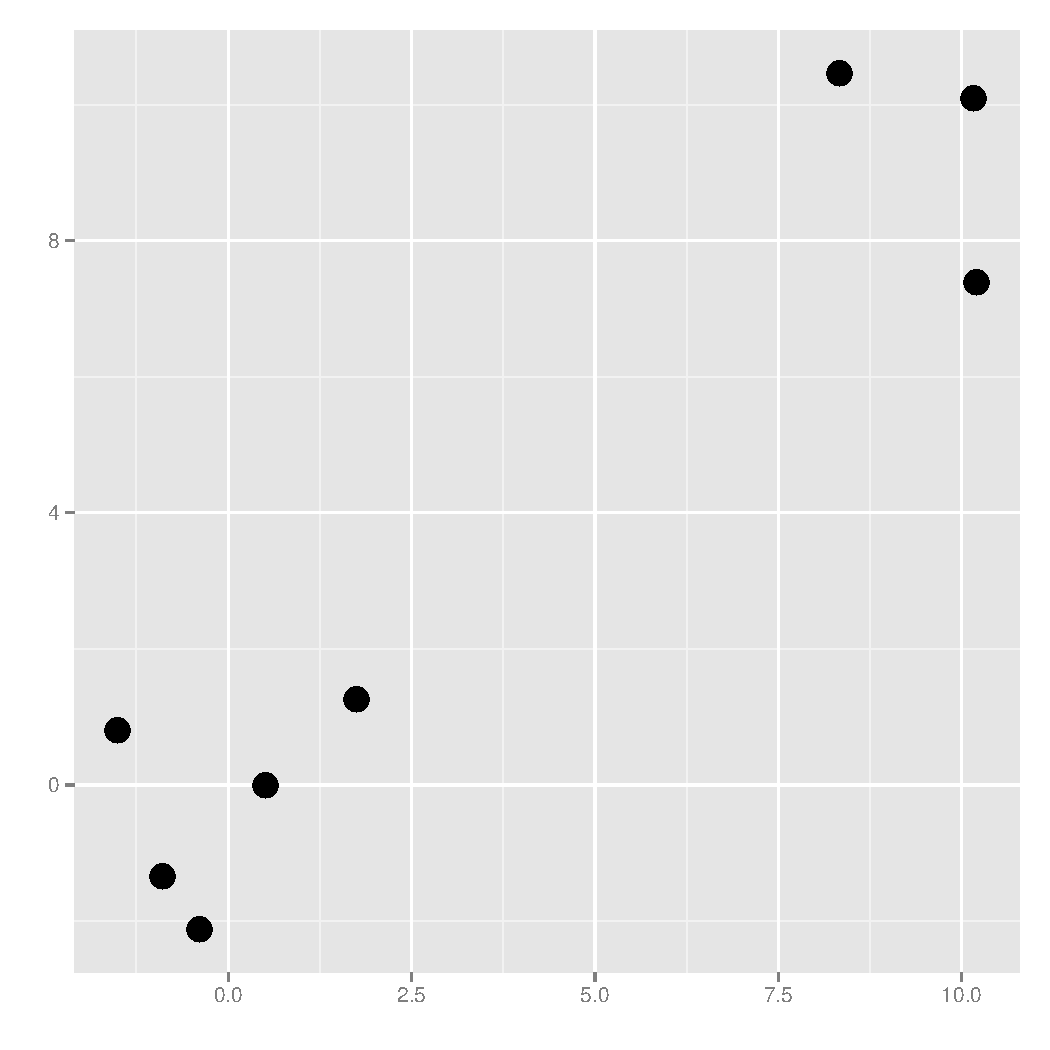
\includegraphics[scale=.2]{../common/pics/kmeans1} 
\end{array}$ 
        $\longrightarrow$  
        $\begin{array}{l}  
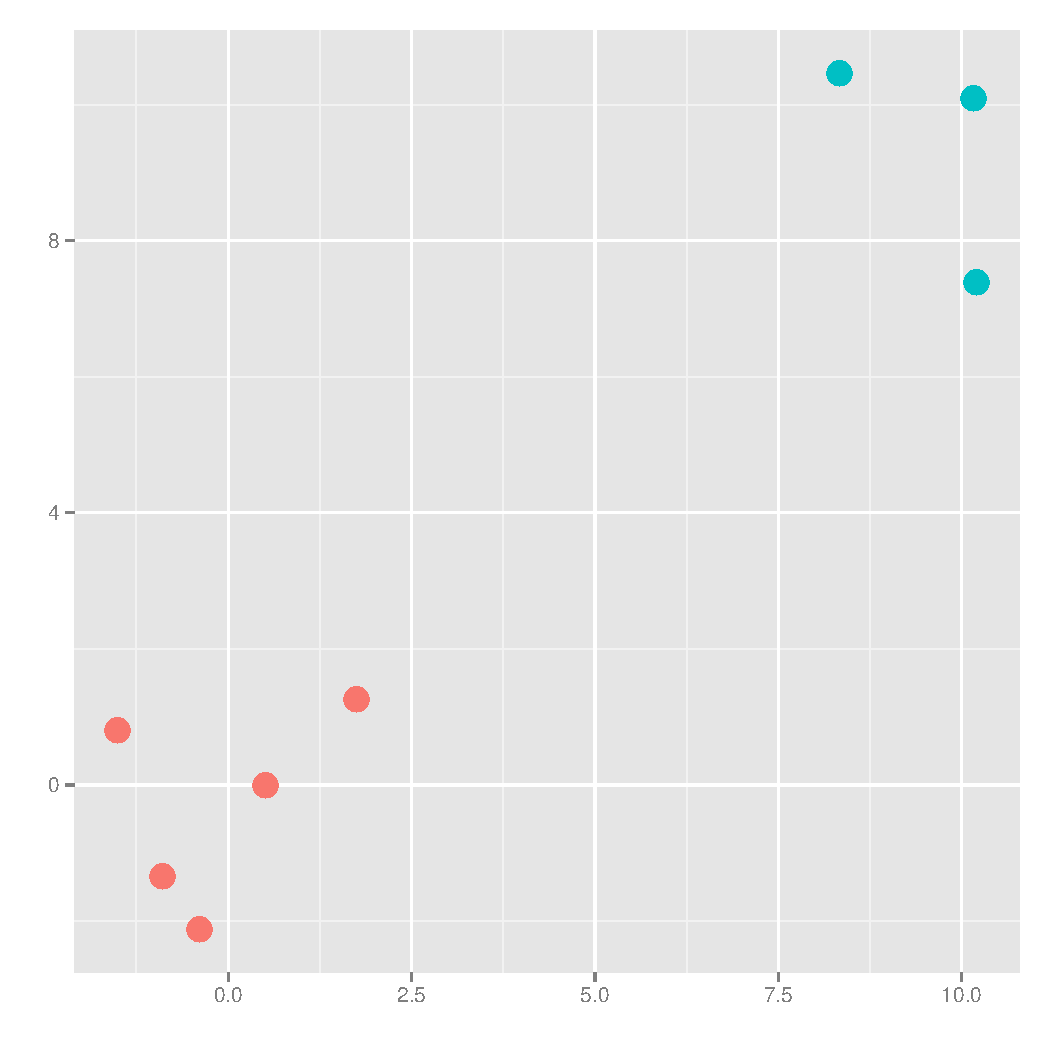
\includegraphics[scale=.2]{../common/pics/kmeans2}\end{array}$
  \end{center}
  
\begin{lstlisting}[backgroundcolor=\color{white},basicstyle=\ttfamily\color{
dkgray}\scriptsize,keywordstyle=\color{black}, 
  commentstyle=\color{orange},stringstyle=\color{mauve}]
R> x <- rbind(matrix(rnorm(5*2, mean=0), ncol=2), 
              matrix(rnorm(3*2, mean=10), ncol=2))
\end{lstlisting}
  \end{exampleblock}
\end{frame}

\begin{frame}[fragile,shrink]
  \begin{exampleblock}{Advanced Statistics (2 of 2): k-Means Clustering}\pause
  \begin{center}
  \end{center}
\vspace{-1cm}
  
\begin{lstlisting}[backgroundcolor=\color{white},basicstyle=\ttfamily\color{
dkgray}\scriptsize,keywordstyle=\color{black}, 
  commentstyle=\color{orange},stringstyle=\color{mauve}]
R> kmeans(x, centers=2)
K-means clustering with 2 clusters of sizes 5, 3

Cluster means:
        [,1]       [,2]
1 -0.1080612 -0.2827576
2  9.5695365  9.3191892

Clustering vector:
[1] 1 1 1 1 1 2 2 2

Within cluster sum of squares by cluster:
[1] 14.675072  7.912641
 (between_SS / total_SS =  93.9 %)

Available components:

[1] "cluster"      "centers"      "totss"        "withinss"     "tot.withinss"
[6] "betweenss"    "size"   
\end{lstlisting}
  \end{exampleblock}
\end{frame}
